%% LyX 2.1.3 created this file.  For more info, see http://www.lyx.org/.
%% Do not edit unless you really know what you are doing.
\documentclass[10pt]{beamer}\usepackage[]{graphicx}\usepackage[]{color}
%% maxwidth is the original width if it is less than linewidth
%% otherwise use linewidth (to make sure the graphics do not exceed the margin)
\makeatletter
\def\maxwidth{ %
  \ifdim\Gin@nat@width>\linewidth
    \linewidth
  \else
    \Gin@nat@width
  \fi
}
\makeatother

\definecolor{fgcolor}{rgb}{0.345, 0.345, 0.345}
\newcommand{\hlnum}[1]{\textcolor[rgb]{0.686,0.059,0.569}{#1}}%
\newcommand{\hlstr}[1]{\textcolor[rgb]{0.192,0.494,0.8}{#1}}%
\newcommand{\hlcom}[1]{\textcolor[rgb]{0.678,0.584,0.686}{\textit{#1}}}%
\newcommand{\hlopt}[1]{\textcolor[rgb]{0,0,0}{#1}}%
\newcommand{\hlstd}[1]{\textcolor[rgb]{0.345,0.345,0.345}{#1}}%
\newcommand{\hlkwa}[1]{\textcolor[rgb]{0.161,0.373,0.58}{\textbf{#1}}}%
\newcommand{\hlkwb}[1]{\textcolor[rgb]{0.69,0.353,0.396}{#1}}%
\newcommand{\hlkwc}[1]{\textcolor[rgb]{0.333,0.667,0.333}{#1}}%
\newcommand{\hlkwd}[1]{\textcolor[rgb]{0.737,0.353,0.396}{\textbf{#1}}}%

\usepackage{framed}
\makeatletter
\newenvironment{kframe}{%
 \def\at@end@of@kframe{}%
 \ifinner\ifhmode%
  \def\at@end@of@kframe{\end{minipage}}%
  \begin{minipage}{\columnwidth}%
 \fi\fi%
 \def\FrameCommand##1{\hskip\@totalleftmargin \hskip-\fboxsep
 \colorbox{shadecolor}{##1}\hskip-\fboxsep
     % There is no \\@totalrightmargin, so:
     \hskip-\linewidth \hskip-\@totalleftmargin \hskip\columnwidth}%
 \MakeFramed {\advance\hsize-\width
   \@totalleftmargin\z@ \linewidth\hsize
   \@setminipage}}%
 {\par\unskip\endMakeFramed%
 \at@end@of@kframe}
\makeatother

\definecolor{shadecolor}{rgb}{.97, .97, .97}
\definecolor{messagecolor}{rgb}{0, 0, 0}
\definecolor{warningcolor}{rgb}{1, 0, 1}
\definecolor{errorcolor}{rgb}{1, 0, 0}
\newenvironment{knitrout}{}{} % an empty environment to be redefined in TeX

\usepackage{alltt}
\usepackage{etex}

\usepackage[T1]{fontenc}
\usepackage{textpos} 
\usepackage{hyperref}
\usepackage{amsmath,amsthm,amsfonts,nicefrac,mathabx,amssymb}
 \usepackage[subnum]{cases}
\usepackage{calligra, mathrsfs}
%\usepackage{natbib}
\usepackage{booktabs}
%\bibpunct{(}{)}{;}{a}{,}{,}
\usepackage[english]{babel}
\usepackage[latin1]{inputenc}
\usepackage{helvet}
\usepackage{graphicx}
\usepackage{color}
\usepackage{multirow,dcolumn}
\usepackage{ragged2e}
\usepackage{xcolor}
\usepackage{colortbl}
\usepackage{booktabs}
\usepackage{enumitem}
\usepackage{url}
\usepackage{bibentry}
\usepackage{chngcntr}

\ifx\hypersetup\undefined
  \AtBeginDocument{%
    \hypersetup{unicode=true,pdfusetitle,
 bookmarks=true,bookmarksnumbered=false,bookmarksopen=false,
 breaklinks=false,pdfborder={0 0 0},backref=false,colorlinks=false}
  }
\else
  \hypersetup{unicode=true,pdfusetitle,
 bookmarks=true,bookmarksnumbered=false,bookmarksopen=false,
 breaklinks=false,pdfborder={0 0 0},backref=false,colorlinks=false}
\fi

\colorlet{tablesubheadcolor}{gray!25}
\colorlet{tableheadcolor}{gray!40}
\colorlet{tablerowcolor}{gray!15.0}
\usetheme{Gesis}
%\setbeamertemplate{navigation symbols}{}
\setbeamertemplate{footline}[frame number]%{\hspace*{.2cm}\insertframenumber}
\setbeamerfont{caption}{size=\footnotesize}
\usefonttheme[onlylarge]{structuresmallcapsserif} % alte Schrift


\definecolor{hellgrau}{rgb}   {0.109375,  0.40625,   0.51953125}
\definecolor{dunkelgrau}{rgb} {0.009375,  0.30625,   0.41953125}
\definecolor{dunkelgrau2}{rgb}{0.009375,  0.20625,   0.31953125}
\definecolor{hellbraun}{rgb}  {0.9140625, 0.8984375, 0.8046875}
\definecolor{hellbraun2}{rgb} {.95,       0.9,       0.8}
\definecolor{alertred}{rgb}   {0.8515625, 0.3828125, 0.08984375}
\definecolor{orange}{rgb}{1,0.5,0}


\setbeamercolor{firstsecslide}{fg=white,bg=dunkelgrau}
\setbeamertemplate{blocks}[rounded][shadow=true]

\newcolumntype{d}[1]{D{.}{.}{#1}}

\newcommand{\emphred}[1]{\textcolor{alertred}{#1}}
\newcommand{\emphcol}[1]{\textcolor{dunkelgrau}{\slshape #1}}

\newcommand{\eqname}[1]{\tag*{#1}} %equation title

\newenvironment{frcseries}{\fontfamily{frc}\selectfont}{}
\newcommand{\textfrc}[1]{{\frcseries#1}}
\newcommand{\mathfrc}[1]{\text{\textfrc{#1}}}


\setcounter{tocdepth}{1}
\setbeamercolor*{section in toc}{fg=hellgrau}
\setbeamertemplate{bibliography item}[default]


\setcounter{secnumdepth}{3}
\setcounter{tocdepth}{3}


\newcommand{\E}[1]{\text{E}\left(#1\right)}
\newcommand{\V}[1]{\text{V}\left(#1\right)}
\newcommand{\Vest}[1]{\widehat{\text{V}}\left(#1\right)}
\newcommand{\MSE}[1]{\text{MSE}\left(#1\right)}
\newcommand{\COV}[2]{\text{COV}\left(#1,\,#2\right)}
\newcommand{\deff}{\ensuremath{\text{\slshape deff}}}
\newcommand{\deffhat}{\ensuremath{\widehat{\text{\slshape deff}}}}
\newcommand{\deffc}{\ensuremath{\text{\slshape deff}_{\text{\slshape c}}}}
\newcommand{\deffhatc}{\ensuremath{\widehat{\text{\slshape deff}}_{\text{\slshape c}}}}
\newcommand{\deffp}{\ensuremath{\text{\slshape deff}_{\text{\slshape p}}}}
\newcommand{\neff}{\ensuremath{n_\text{\slshape eff}}}
\newcommand{\nnet}{\ensuremath{n_\text{\slshape net}}}
\newcommand{\ngross}{\ensuremath{n_\text{\slshape gross}}}
%roman numbers in equation
\newcommand{\RN}[1]{%
  \textup{\uppercase\expandafter{\romannumeral#1}}%
}


\makeatletter

\addtobeamertemplate{frametitle}{}{%
\begin{textblock*}{100mm}(.91\textwidth,-1cm)

\includegraphics[height=1cm,width=2cm]{graphs/logos/GESIS_Logo_kompakt_en.jpg}
\end{textblock*}}



%%%%%%%%%%%%%%%%%%%%%%%%%%%%%% LyX specific LaTeX commands.
\providecommand{\LyX}{\texorpdfstring%
  {L\kern-.1667em\lower.25em\hbox{Y}\kern-.125emX\@}
  {LyX}}

%%%%%%%%%%%%%%%%%%%%%%%%%%%%% Textclass specific LaTeX commands.
% this default might be overridden by plain title style
 \newcommand\makebeamertitle{\frame{\maketitle}}%
 % (ERT) argument for the TOC
 \AtBeginDocument{%
   \let\origtableofcontents=\tableofcontents
   \def\tableofcontents{\@ifnextchar[{\origtableofcontents}{\gobbletableofcontents}}
   \def\gobbletableofcontents#1{\origtableofcontents}
 }

%%%%%%%%%%%%%%%%%%%%%%%%%%%%%% User specified LaTeX commands.
%\usetheme{Montpellier}%\usetheme{PaloAlto}

\makeatother
\IfFileExists{upquote.sty}{\usepackage{upquote}}{}
\begin{document}



\title[Complex Sampling Designs]{Sampling and Estimation}   
\subtitle{Day 2: Complex Sampling Designs}

\author{Stefan Zins\thanks{\href{mailto:Stefan.Zins@gesis.org}{Stefan.Zins@gesis.org}} and Matthias Sand\thanks{\href{mailto:Matthias.Sand@gesis.org}{Matthias.Sand@gesis.org}}}
\date{\today} 

\makebeamertitle

%Picture for cluster sampling

\begin{frame}{Clustering}

A Population of 100 elements is clustered into $N_{\RN{1}}=6$ cluster
%fig.keep='all',fig.show='asis'
\onslide*<1>{
\begin{knitrout}\footnotesize
\definecolor{shadecolor}{rgb}{0.969, 0.969, 0.969}\color{fgcolor}

{\centering 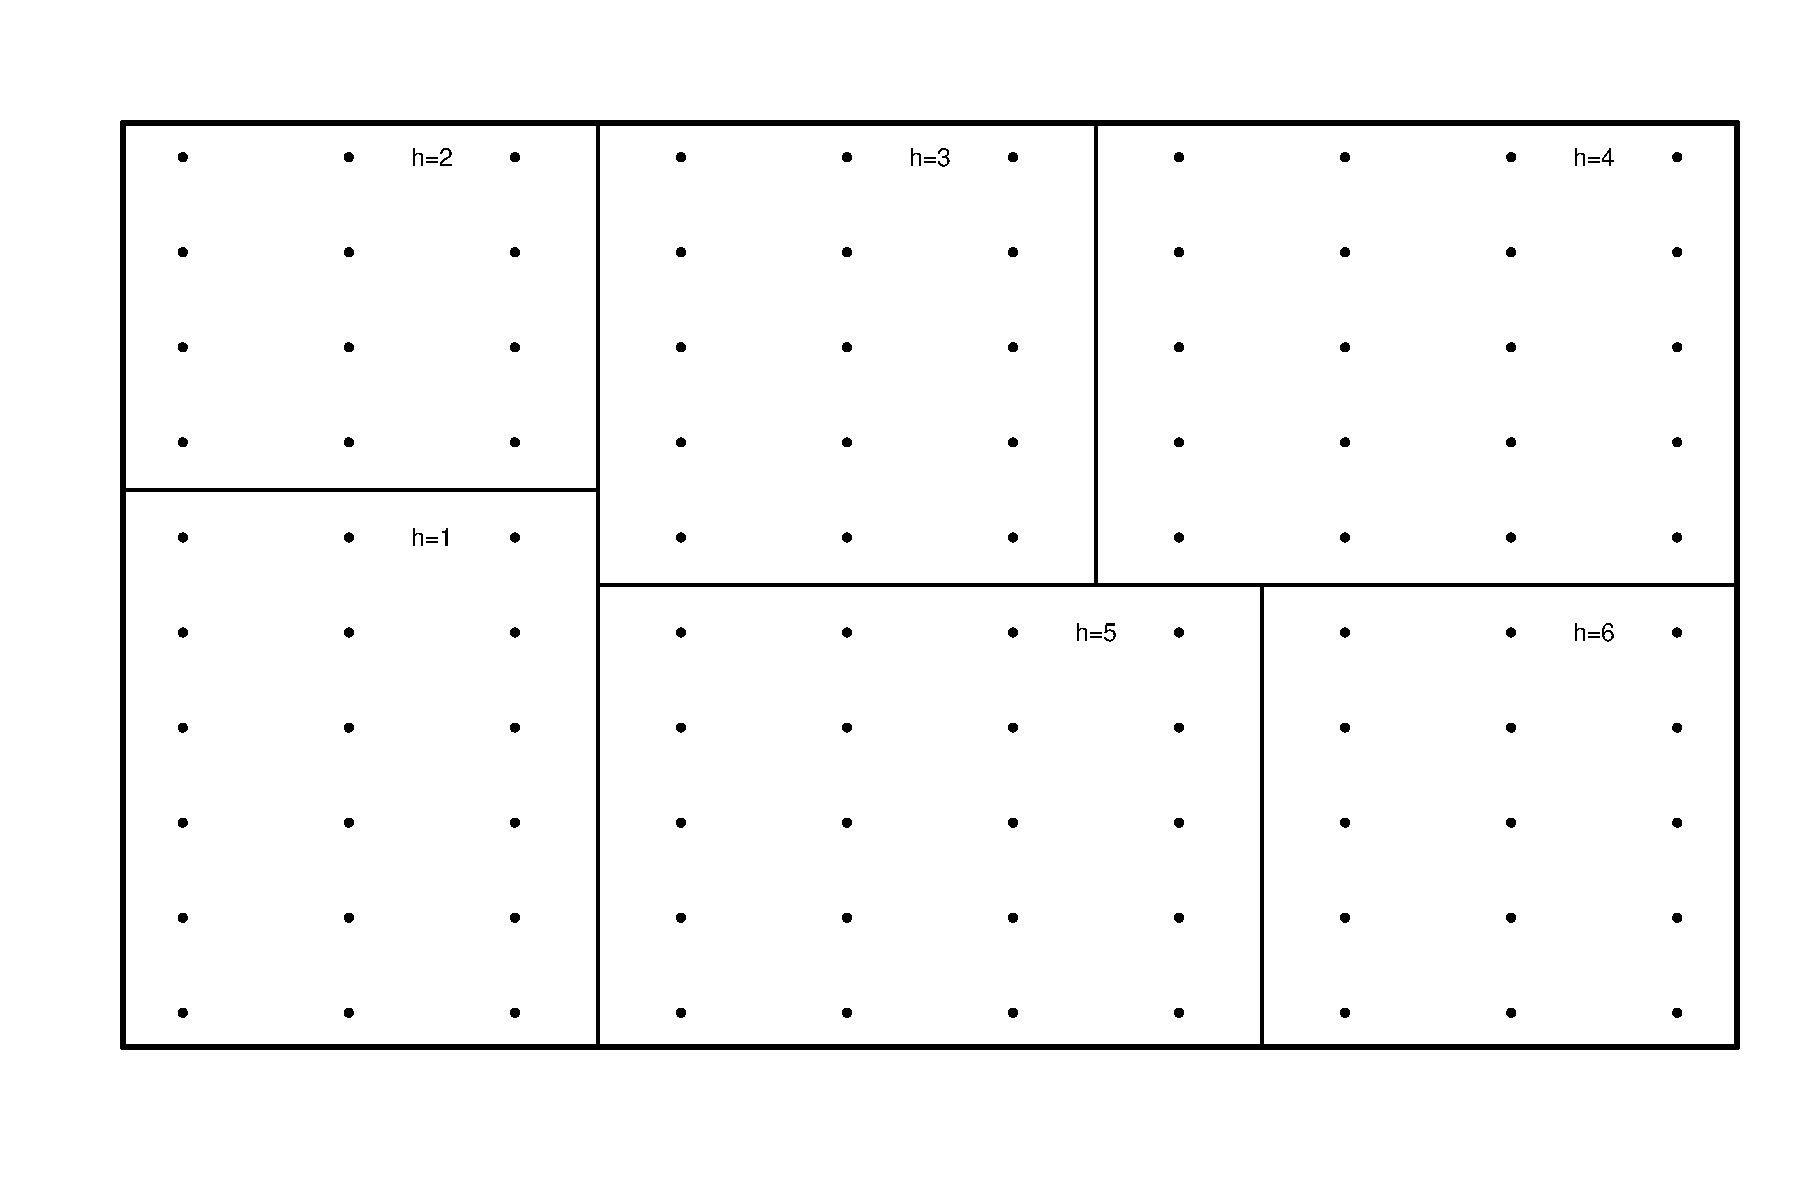
\includegraphics[width=.85\linewidth]{graphs/beamer-StratPlot1-1} 

}



\end{knitrout}
}\onslide<2>{
and $n_{\RN{1}}=2$ clusters are selected from the population.
\begin{knitrout}\footnotesize
\definecolor{shadecolor}{rgb}{0.969, 0.969, 0.969}\color{fgcolor}

{\centering 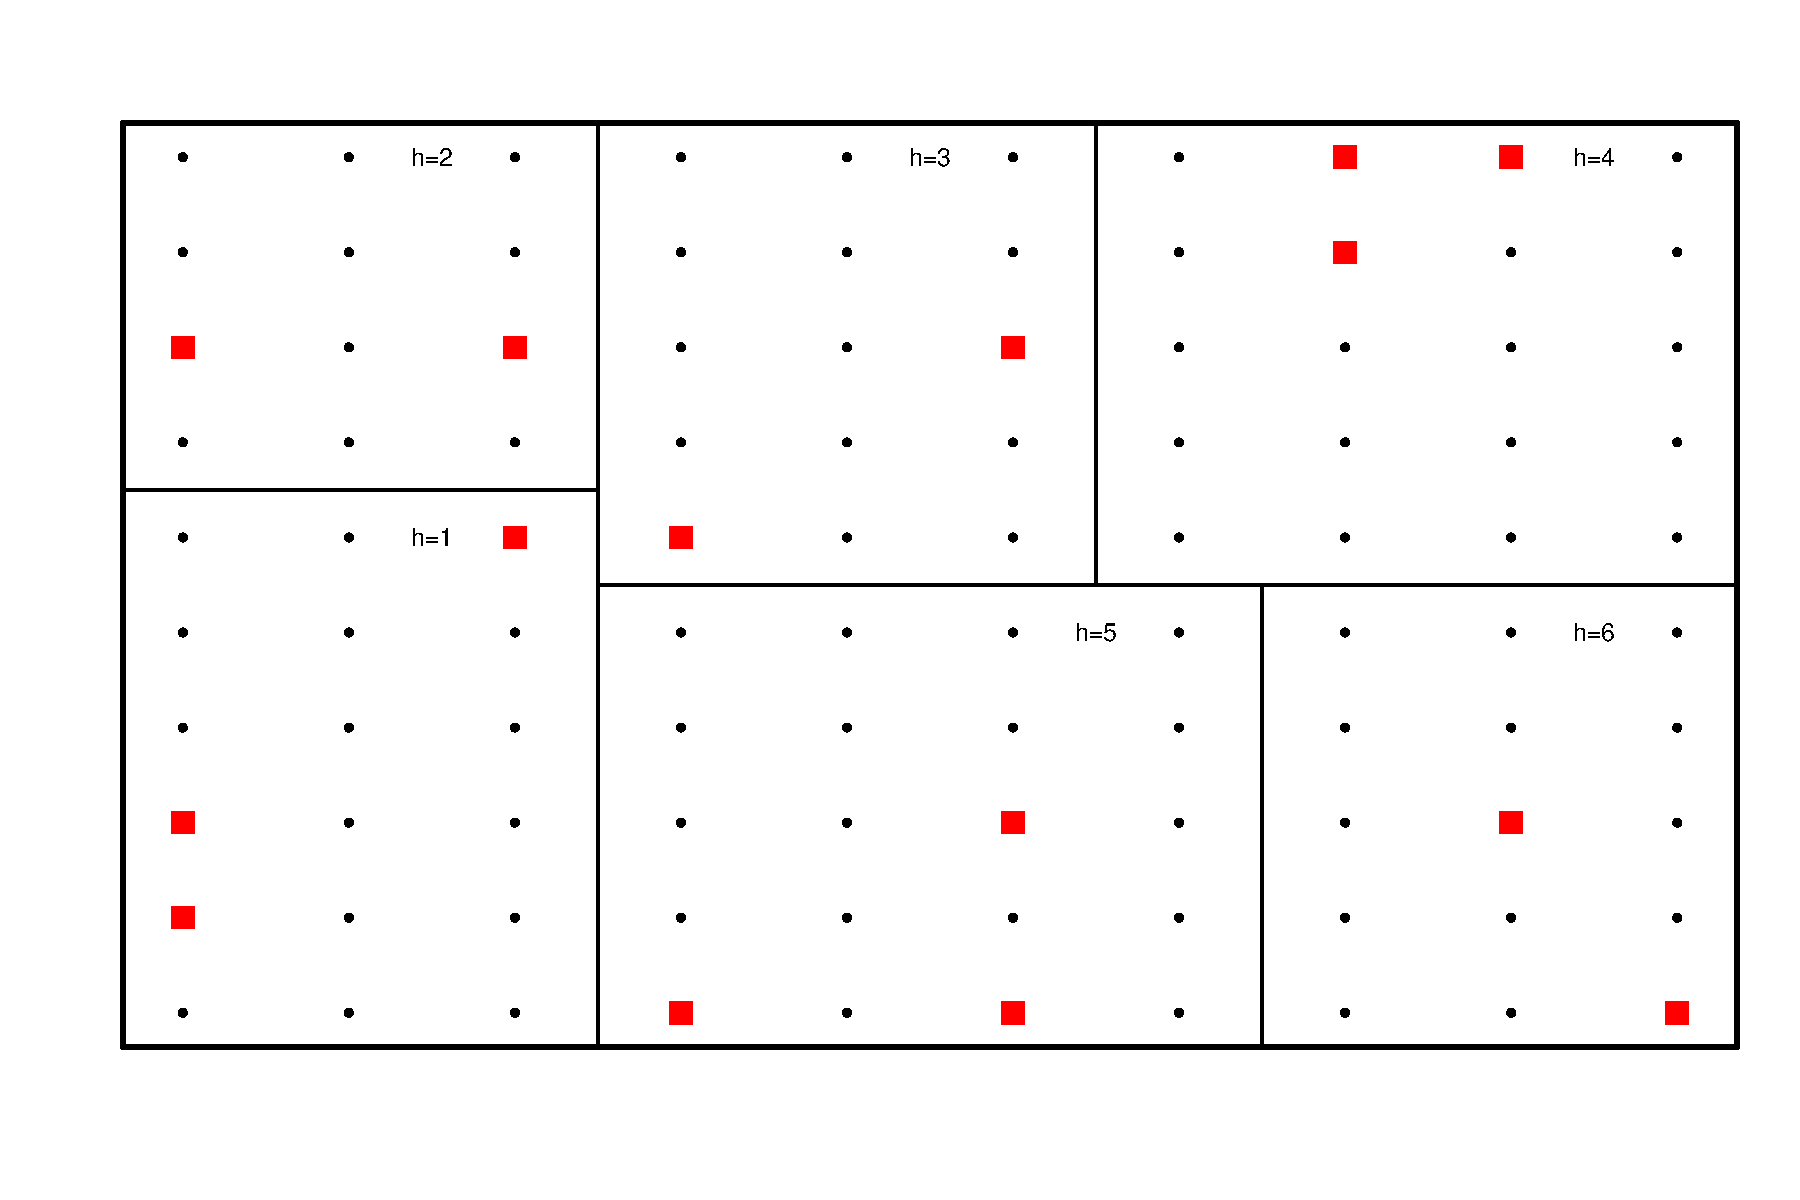
\includegraphics[width=.85\linewidth]{graphs/beamer-StratPlot2-1} 

}



\end{knitrout}
}
\end{frame}


\begin{frame}{Cluster Sampling}
\begin{itemize}
\item[]<1-> Sampling elementary units is often not feasible (e.g. persons or businesses). Maybe there is no uniform sampling frame available to select them from, or it would be costly to do, because the selected elements would scatter to much over the a certain area and travel costs of interviewers would be to high. 

\item[]<2-> Thus, it is very common to select clusters, so called \emph{primary sampling units} (PSU's) that are populated by \emph{secondary sampling units} (SSU's).

\item[]<3-> Cluster sampling makes it still possible to obtain unbiased estimates but it can have a big influence on the variance. 
\end{itemize}

\end{frame}


\begin{frame}{Notation}
\begin{tabular}{rcp{8cm}}
$y_{ki}$      &=&value of the variable of interest for the $k$-th SSU in the $i$-th PSU \\
$N_{\RN{1}}$     &=&number of PSU's in the population \\
$N_i$       &=&number of SSU's in the $i$-th PSU \\
$N$         &=&total number of SSU's in the Population \\
$\mathcal{U}$  &=& set of SSU's in the population \\
$\mathcal{U}_{\RN{1}} $  &=& set of PSU's in the population \\
$\mathcal{U}_i$  &=& set of SSU's in the $i$-th PSU \\
$n_{\RN{1}}$         &=&number of PSU's in the sample \\
$n_i$   &=&number of SSU's in the sample from the $i$-th PSU\\
$\mathfrc{s}_{\RN{1}}$  &=& sample of PSU's \\
$\mathfrc{s}_i$         &=& sample SSU's from the $i$-th PSU \\ 
$p_{\RN{1}}(.)$         &=& sampling design of the PSU's \\
\end{tabular}

\end{frame}

\begin{frame}{Estimation in Case of $p_{\RN{1}}(.)=$ SRS}
All SSU's in the sampled PSU's are surveyed, thus
$$\tau_i=\sum_{k \in \mathcal{U}_i} y_{ki}$$
is known of all selected PSU's.
An unbiased estimator for the population mean is
$$\overline{y}_{\text{SRCS}} = \dfrac{N_{\RN{1}}}{N}  \sum_{i \in  \mathfrc{s}_{\RN{1}}}   \dfrac{\tau_i}{n_{\RN{1}}} $$
\onslide*<1>{with variance
$$\V{\overline{y}}_{\text{SRCS}} = \dfrac{N_{\RN{1}}^2}{N^2}  \left( 1 - \dfrac{n_{\RN{1}}}{N_{\RN{1}}} \right) \dfrac{V^2_{\tau}}{n_{\RN{1}}}\;,$$
where
 $V^2_{\tau} = \dfrac{1}{N_{\RN{1}} - 1} \sum_{i \in \mathcal{U}_{\RN{1}}} \left(\tau_i - \mu_\tau \right)^2$
and
 $\mu_\tau = \sum_{i \in \mathcal{U}_{\RN{1}}} \dfrac{\tau_i}{N_{\RN{1}}}$.
 }
\onslide*<2>{An unbiased variance estimator is
$$\Vest{\overline{y}_{\text{SRCS}}}_{\text{SRS}} = \dfrac{N_{\RN{1}}^2}{N^2} \left( 1 - \dfrac{n_{\RN{1}}}{N_{\RN{1}}} \right) \dfrac{s^2_{\tau}}{n_{\RN{1}}}\;,$$
where 
 $$
 s^2_{\tau} = \dfrac{1}{n_{\RN{1}}-1} \sum_{i \in \mathfrc{s}_{\RN{1}} } \left( \tau_i - \overline{\tau}  \right)^2\;.
 $$
with $\overline{\tau}=\sum_{i \in \mathfrc{s}_{\RN{1}} } \frac{\tau_i}{ n_{\RN{1}} }$. 
}
\end{frame}

\begin{frame}
\frametitle{Simple Cluster Sampling}
\onslide<1->{
% latex table generated in R 3.2.2 by xtable 1.7-4 package
% Wed Jan 13 13:31:04 2016
\begin{table}[ht]
\centering
\caption{Two Variations of a Population Composed of 5
clusters of Size 5} 
\begin{tabular}{r|rrrrr|r|r}
  & 1 & 2 & 3 & 4 & 5 & $\mu_{i.}$ & $V^2_{i.}$ \\ 
  \hline
1 & 1.0 & 2.0 & 3.0 & 4.0 & 5.0 & 3.0 & 2.5 \\ 
  2 & 6.0 & 7.0 & 8.0 & 9.0 & 10.0 & 8.0 & 2.5 \\ 
  3 & 11.0 & 12.0 & 13.0 & 14.0 & 15.0 & 13.0 & 2.5 \\ 
  4 & 16.0 & 17.0 & 18.0 & 19.0 & 20.0 & 18.0 & 2.5 \\ 
  5 & 21.0 & 22.0 & 23.0 & 24.0 & 25.0 & 23.0 & 2.5 \\ 
   \hline
$\mu_{.j}$ & 11.0 & 12.0 & 13.0 & 14.0 & 15.0 & 13.0 &  \\ 
   \hline
$V^2_{.j}$ & 62.5 & 62.5 & 62.5 & 62.5 & 62.5 &  & 54.2 \\ 
  \end{tabular}
\end{table}

We have homogeneity of means between columns and heterogeneity of means between rows.
}
\onslide<2>{Sample $n=10$ SSU's by
\begin{enumerate}[label=\arabic*)]
\item SRS n=10
\item Simple random cluster sampling $n_{\RN{1}}=2$
\begin{enumerate}[label=\alph*)]
 \item columns
 \item rows
\end{enumerate}
\end{enumerate}
}
\end{frame}

\begin{frame}
	\frametitle{Simple Cluster Sampling}
	 Comparing the mean and variance of $\overline{y}$ and $\overline{y}_{\text{SRCS}}$ after 100,000 samples:
% latex table generated in R 3.2.2 by xtable 1.7-4 package
% Wed Jan 13 13:31:08 2016
\begin{table}[ht]
\centering
\caption{Results from the Simulation Study} 
\begin{tabular}{l|rrr}
  & SRS & SRCS a & SRCS b \\ 
  \hline
mean & 13.0 & 13.0 & 13.0 \\ 
  var & 3.2 & 0.8 & 18.9 \\ 
  \end{tabular}
\end{table}

\onslide<2->{True values:
\begin{tabular}{l c d{1} l}
$\mu $ & =& 13 & \\
$\V{\overline{y}}_{\text{SRS}}$ &=& 3.25	&  SRS \\
$\V{\overline{y}_{\text{SRCS}}}_{\text{SRS}}$  &=& 0.75   & SRCS  a \\
 $\V{\overline{y}_{\text{SRCS}}}_{\text{SRS}}$ &=& 18.75   &  SRCS b \\
\end{tabular} \newline
Bias is not an issue, however variance is. 
}
\onslide<3->{\newline
If the cluster where strata, which stratification would you use, columns or rows?}
\onslide<4->{\newline What good is for stratified sampling, i.e. low SSW, is bad of cluster sampling and vice versa.}
\end{frame}


\begin{frame}{Tow Stage Sampling}
A Population of 100 elements is clustered into $N_{\RN{1}}=6$ clusters
and $n_{\RN{1}}=2$ clusters (PSU) are selected at the first sampling stage
\onslide*<1>{
\begin{knitrout}\footnotesize
\definecolor{shadecolor}{rgb}{0.969, 0.969, 0.969}\color{fgcolor}

{\centering 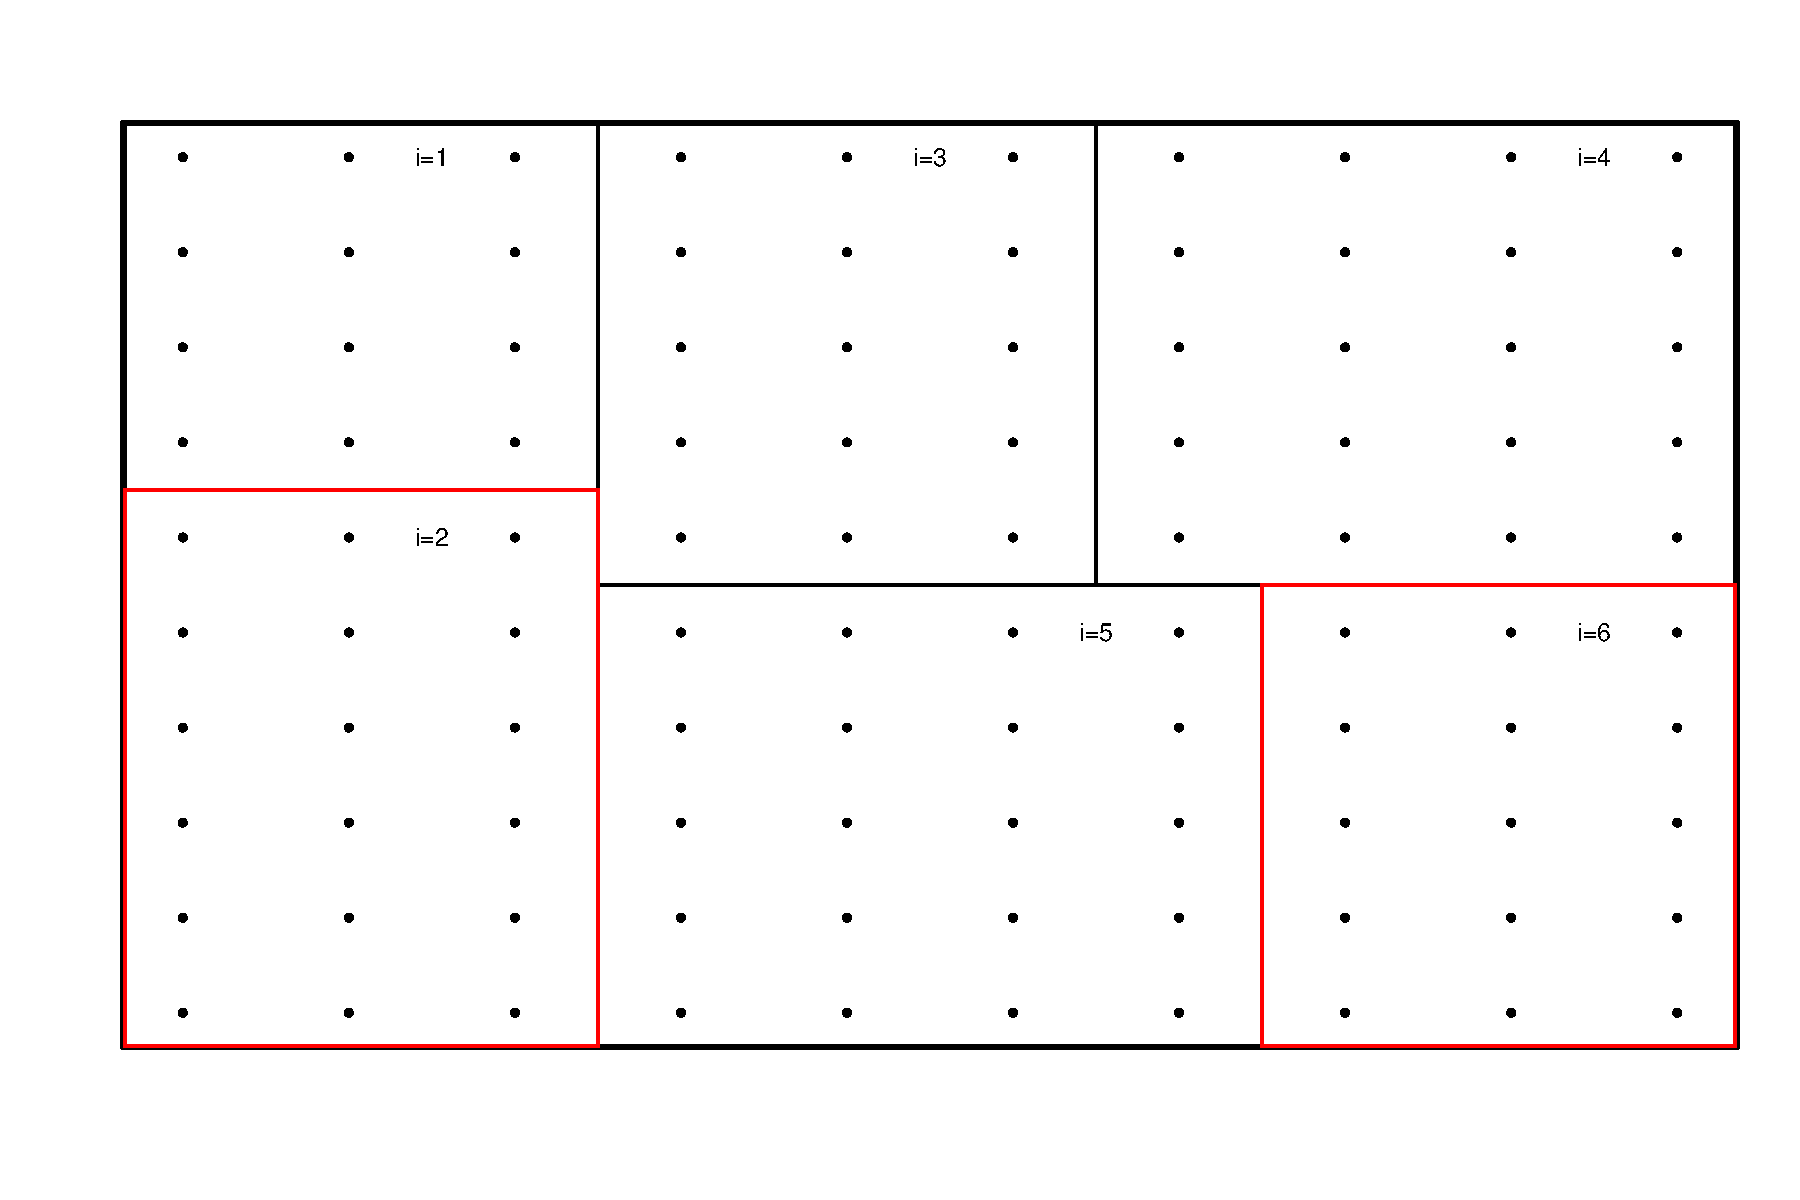
\includegraphics[width=.85\linewidth]{graphs/beamer-StratPlot1_2-1} 

}



\end{knitrout}
}\onslide<2>{
and $n_{i}=4$ elements are selected from each sampled cluster.
\begin{knitrout}\footnotesize
\definecolor{shadecolor}{rgb}{0.969, 0.969, 0.969}\color{fgcolor}

{\centering 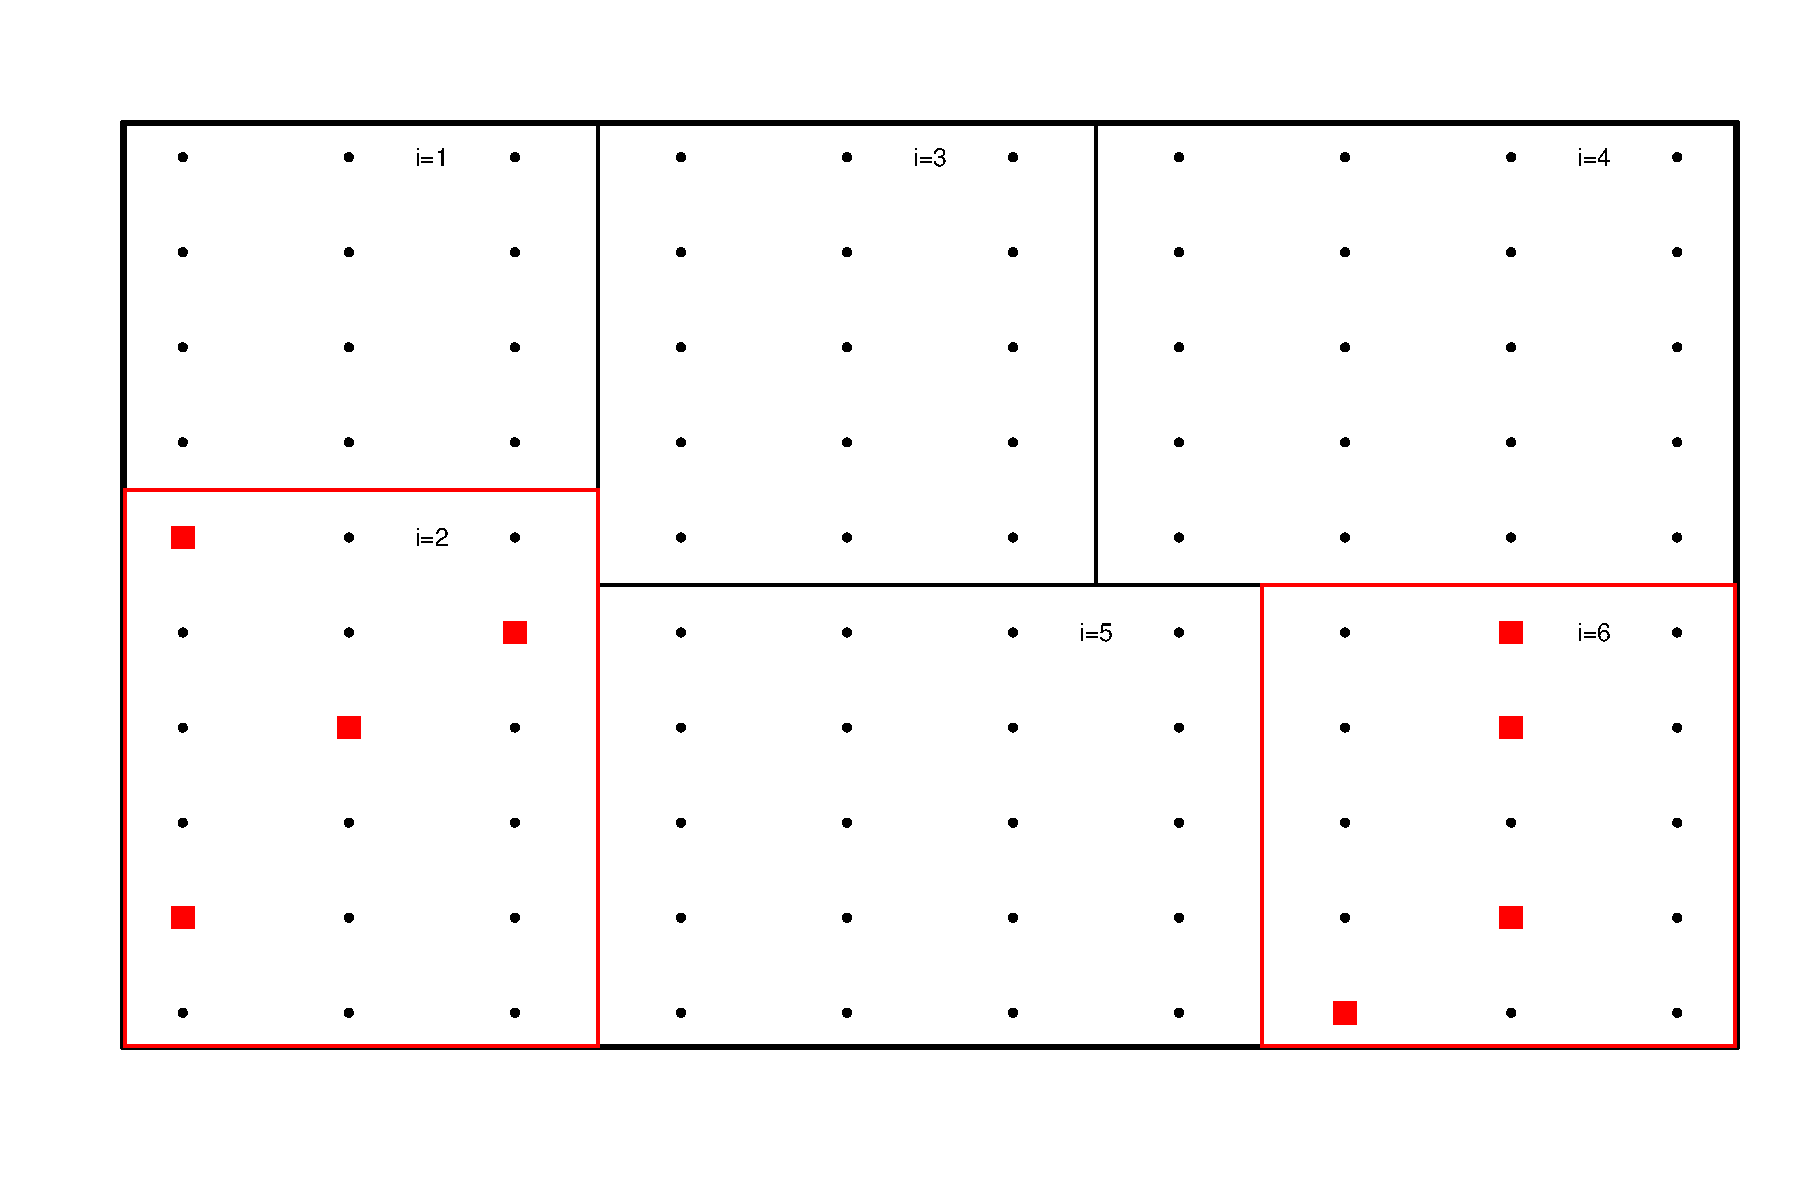
\includegraphics[width=.85\linewidth]{graphs/beamer-StratPlot2_2-1} 

}



\end{knitrout}
}
  




\end{frame}


\begin{frame}{Two Stage Sampling}
 \begin{description}
 \item[First  stage] A sample $\mathfrc{s}_{\RN{1}}$ of PSU's is drawn from $\mathcal{U}_{\RN{1}}$ according to some sampling design $p_{\RN{1}}(.)$
 \item[Second stage] For every $i \in \mathfrc{s}_{\RN{1}}$ a sample $\mathfrc{s}_i$ of SSU's is selected from $\mathcal{U}_i$ according to some design $p_i(.|\mathfrc{s}_{\RN{1}})$
 \end{description}
 The resulting sample of SSU's is denote $\mathfrc{s}= \bigcup_{i \in \mathfrc{s}_{\RN{1}}} \mathfrc{s}_i $.
 In general samples $\mathfrc{s}_i$ are selected independently of each other, thus the inclusion probability of a element $k \in \mathcal{U}_i$ is
$$\pi_k=\pi_{\RN{1}i}\pi_{k|i}\;,$$
where $\pi_{\RN{1}i}$ is the probability of selecting the $i$-th PSU and $\pi_{k|i}$  the probability of selecting
the $k$-th SSU in the $i$-th PSU.
\end{frame}


\begin{frame}{Estimation Simple Random Tow Stage Sampling}
Designs $p_{\RN{1}}(.)$ and $p_i(.|\mathfrc{s}_{\RN{1}})$ are both SRS.
Since not all SSU's in the sampled PSU's are surveyed  $\tau_i$ has to be estimated by $\hat{\tau}_i = \frac{N_i}{n_i} \sum_{k \in \mathfrc{s}_i} y_{ki} $.
An unbiased estimator for the population mean is
$$ \overline{y}_{\text{2SRS}} = \dfrac{N_{\RN{1}}}{N}  \sum_{i \in  \mathfrc{s}_{\RN{1}}}   \dfrac{\hat{\tau}_i}{n_{\RN{1}}} $$
\onslide*<2>{with variance
$$
\V{\overline{y}_{\text{2SRS}}}_{\text{SRS}} = \dfrac{1}{N^2}  \left( N_{\RN{1}}^2  \left( 1 - \dfrac{n_{\RN{1}}}{N_{\RN{1}}} \right) \dfrac{V^2_{\tau}}{n_\RN{1}} + \dfrac{N_{\RN{1}}}{n_{\RN{1}}} \sum_{i \in \mathcal{U}_{\RN{1}}} N_i^2 \left( 1 - \dfrac{n_i}{N_i} \right) \dfrac{V_{i}^2}{n_i} \right) \;,
$$
where $V_{i}^2 = \frac{1}{N_i-1} \sum_{k \in \mathcal{U}_i} (y_{ki} - \mu_i )^2$ with $\mu_i = \sum_{k \in \mathcal{U}_i} \dfrac{y_{ki}}{N_i}$.
}\onslide*<3>{An unbiased variance estimator is given by
$$
\Vest{\overline{y}_{\text{2SRS}}}_{\text{SRS}} =  \dfrac{1}{N^2}  \left( N_{\RN{1}}^2  \left( 1 - \dfrac{n_{\RN{1}}}{N_{\RN{1}}} \right) \dfrac{s^2_{\hat{\tau}}}{n_\RN{1}} + \dfrac{N_{\RN{1}}}{n_{\RN{1}}} \sum_{i \in \mathfrc{s}_{i}} N_i^2 \left( 1 - \dfrac{n_i}{N_i} \right) \dfrac{s_{i}^2}{n_I}  \right) \;,
$$
where $s^2_{\hat{\tau}}=\frac{1}{n_{\RN{1}}-1} \sum_{i \in \mathfrc{s}_{\RN{1}} } (\hat{\tau}_i  - \overline{\hat{\tau}} )^2$
with $\overline{\hat{\tau}} = \sum_{i \in \mathfrc{s}_{\RN{1}} }\frac{\hat{\tau}_i}{n_{\RN{1}}}$ and 
$s^2_{i} = \frac{1}{n_{i}-1}  \sum_{k \in \mathfrc{s}_{i} } (y_{ki}  - \overline{y}_i )^2$
with $\overline{y}_i  = \sum_{k \in \mathfrc{s}_{i} } \frac{y_{ki}}{n_i}$.

}
%Note: For $M_i = n_i$ we are back to SRCS.
\end{frame}


\begin{frame}{Unequal Probability Sampling I}
There are good reasons to deviate from the simple selection procedure that gives every unit the same inclusion probability. If good prior information is available its incorporation into the sampling design can dramatically improve the efficiency of an estimator.
\begin{itemize}
 \item An optimal allocation would be favorable to a proportional allocation.
 \item Selecting the elements proportional to a variable that is correlated to the variable of interest can greatly improve the quality of estimates.
\end{itemize}

There are many techniques (i.e. sampling algorithms) to select elements with unequal probabilities [Till\'e, 2006].
% Some of them have variable sample sizes (e.g. Poisson Sampling), other have but
% 
% Possion Sampling simple but  
% Systematic Sampling
% Sampford simple not

\end{frame}


\begin{frame}{A Generic Design Based Estimator}
A design unbiased estimator for the total $\tau=\sum_{k \in \mathcal{U}} y_k$ is given by
\begin{gather*}
 \hat{\tau}_{\pi} = \sum_{k \in \mathfrc{s}} \dfrac{y_k}{\pi_k} \;,
\end{gather*}
which is also known as \emph{Horvitz-Thompson} (HT) or $\pi$-estimator.
%Assuming a design with strictly positive second order inclusion probabilities
\onslide*<2>{
The variance of $ \hat{\tau}_{\pi} $ is 
\begin{align*}
 \V{ \hat{\tau}_{\pi}} = \sum_{k \in \mathcal{U}} \sum_{l \in \mathcal{U}} \left( \pi_{kl} - \pi_k \pi_l \right)
\dfrac{y_k}{\pi_k}\dfrac{y_l}{\pi_l} \;,
\end{align*}
which can be estimated by
\begin{align*}
 \Vest{ \hat{\tau}_{\pi}}_1 = \sum_{k \in \mathfrc{s}} \sum_{l \in \mathfrc{s}} \dfrac{\left( \pi_{kl} - \pi_k \pi_l \right)}{\pi_{kl}} \dfrac{y_k}{\pi_k}\dfrac{y_l}{\pi_l} \;.
\end{align*}
}\onslide*<3->{
For a fixed size design we may write the variance of $\hat{\tau}_{\pi}$ as
\begin{align*}
 \V{ \hat{\tau}_{\pi}} = - \dfrac{1}{2} \sum_{k \in \mathcal{U}} \sum_{l \in \mathcal{U}} \left( \pi_{kl} - \pi_k \pi_l \right) \left(\dfrac{y_k}{\pi_k} - \dfrac{y_l}{\pi_l}\right)^2 \;,
\end{align*}
which can be estimated by
\begin{align*}
 \Vest{ \hat{\tau}_{\pi}}_2 = - \dfrac{1}{2} \sum_{k \in \mathfrc{s}} \sum_{l \in \mathfrc{s}} \dfrac{\left( \pi_{kl} - \pi_k \pi_l \right)}{\pi_{kl}} \left(\dfrac{y_k}{\pi_k} - \dfrac{y_l}{\pi_l}\right)^2 \;.
\end{align*}
}
\onslide*<4>{Provided that $\pi_{kl} > 0$ for all $k \neq l \in \mathcal{U}$ both variance estimators are unbiased. Nevertheless both variance estimators can become negative!}
\end{frame}


\begin{frame}{Unequal Probability Sampling II}
If there is some prior information available in the form of a variable $\mathcal{X} =  \{ x_1{,}x_2{,}\,\ldots{,}\,x_k{,}\,\ldots{,}\,x_N \}$ which is correlated to our variable interest $\mathcal{Y}$ we can select elements proportional to it

$$\nu_k = \dfrac{x_k}{\sum_{k \in \mathcal{U}} x_k} n \;.$$
Unequal inclusion probabilities can reduce the variance of an estimator, \emph{if} they are related to the variable of interest. We may have $\nu_k=\pi_k$ but in general $\nu_k$ can be greater than 1. \newline

For instance, to estimate the sales in an industry, sampling companies or business with equal probabilities might be bad idea. It would be better to sample companies proportional to a variable that is related to their sales, say their number of employee. That way there is a much higher chance to included the biggest companies into the sample that accumulate the major share of the sales. \newline

Note: In the extreme case if $\pi_k = \alpha y_k$, with  $\alpha \in \mathbb{R}$, for all $k \in \mathcal{U}$ and we have a fixed size design  $\V{ \hat{\tau}_{\pi}}$ would even be zero.

\end{frame}


\begin{frame}{Systematic Sampling with \\ Unequal Inclusion Probabilities}
Again the elements of the population are brought into a specific ordered and $V^i = \sum_{k=1}^i \pi_k$. Then $\lambda_k$ is drawn from a uniform distribution between $0$ and $1$.
~\\[-4cm]
\begin{knitrout}\footnotesize
\definecolor{shadecolor}{rgb}{0.969, 0.969, 0.969}\color{fgcolor}

{\centering 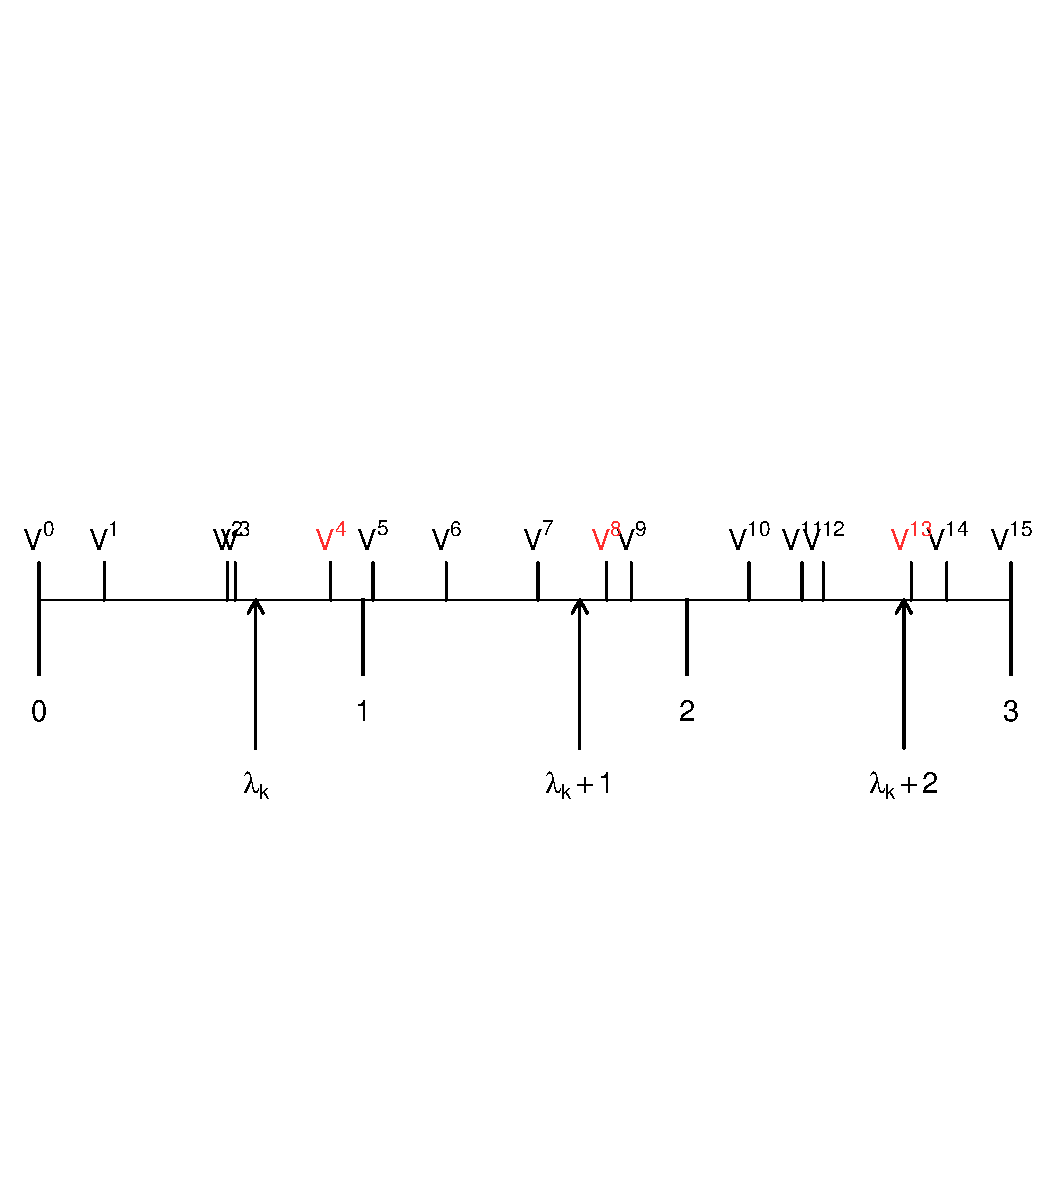
\includegraphics[width=.95\linewidth]{graphs/beamer-UP_SYS-1} 

}



\end{knitrout}
~\\[-4cm]
Systematic selection remains popular because of its simplicity. Also it can easily be applied to the case where an element can be selected more than one time, i.e. $\pi_k \neq \nu_k > 1$. Then we would use $V^i = \sum_{k=1}^i \nu_k$.

\end{frame}


\begin{frame}{A Typical Sample of Persons}{in Germany}
\onslide*<1>{A two-stage Sampling Design:

\begin{description}
\item[First Stage] Municipalities are the PSU's. The sampling design for the PSU's is a stratified design with an allocation proportional to the population within each stratum (not number of PSU's). Within the strata PSU's are sampled proportional to their population size.
\item[Second Stage] Persons are the SSU's. The SSU's are selected form the 	population register of the  municipalities by a simple systematic sample.
\end{description}

}
\onslide*<2>{
\begin{itemize}
\item Very large municipalities, (e.g. Berlin), are selected with certainty, this happens if
$\nu_i = \dfrac{N_i}{N} n_{\RN{1}} > 1$. The integer part of $\nu_i$ indicates how many sampling points are \emph{at least} associated with a municipalities. A sampling point is here a multiplier, indicating how many times $n_i$ SSU's are selected from the $i$-th PSU, where $n_i$ is usually fix for all PSU's.

\item For instance, $\nu_i=3.4$, means that the $i$-th PSU will always be in the sample with at least 3 sampling points, but with a probability of $0.4$ it can be in the sample with 4 sampling points.
\end{itemize}
}

\onslide<3->{Has this design equal inclusion probabilities? \newline}\onslide<4>{Yes, if for each sampling point the same number of SSU's $n_{\ast}$ is sampled. Because 
$$\dfrac{N_i}{N} n_{\RN{1}} \times \dfrac{n_{\ast}}{N_i} = \dfrac{n_{\RN{1}} n_{\ast}}{N} \;.$$
Note that $n_{\RN{1}}$ is not the size of the PSU sample, but the number of sampling points, which can be higher.
}

\end{frame}



%Also the 
\begin{frame}{On Complex Sampling Design}
\begin{itemize}
\item<1|only@1> Selecting PSU's or clusters proportional to some size measure is very common.
This however does not mean that the inclusion probabilities of elementary units are unequal.

\item<2|only@2>  The concept of two-stage designs can also be extended to three, four, or more stages.
The principle of such multi-stage design remains the same, select clusters then select again within clusters.

\item<3|only@3>  There are many ways to optimize the sampling design with respect to one particular goal, i.e. the estimation of a specific statistic. However, it becomes difficult to optimize a design and at the same time retain a balance for a maximum of possible applications, which is a problem when planning a multipurpose survey that has a multitude of variables and covers different topics.
Thus simple design,  such as SRS or StrSRS, are justifiable, as these designs are robust towards any possible analysis of the sample data.

\item<4|only@4>  Multi-stage sampling is usually not a matter of choose but done out of necessity.

\item<5|only@5>  Most importantly, the same design weights ($\pi_k^{-1}$) do \emph{not} imply the same sampling variance. Different designs can be used to select samples with same $\pi_k$'s, however their $\pi_{kl}$'s might be very different and so is their associated sampling variance.

\end{itemize}

\end{frame}

\section{Design Effect}

\begin{frame}\frametitle{The Design Effect}
 The design effect compares strategies, i.e. a combination of a sampling design and an estimator.

	If $p(.)$ is some other design than SRS, however with $\sum_{i=1}^N \pi_k$ equal to the sample size $n$ of the SRS design, then the \emph{design effect} for strategy $(p(.) ,\, \hat{\tau}_{\pi})$ can be defined as
	 $$ \deff(p, \hat{\tau}_{\pi}) = \dfrac{\V{\hat{\tau}_{\pi}}_p}{\V{ \hat{\tau}_{\pi}}_{\text{SRS}}} = 
	  \dfrac{\sum_{k=1}^N \sum_{l=1}^N  \left(\pi_{kl}  - \pi_k \pi_l \right) \dfrac{y_k}{\pi_k}\dfrac{y_l}{\pi_l}}{N^2 \left( 1 - \dfrac{1}{N} \right) \dfrac{V^2}{n} }\;{.} 
	 $$
	The design effect $\deff(p, \hat{\tau}_{\pi})$ expresses how well a design $p(.)$ fares in comparison to reference design SRS.

	\begin{itemize}
		\item $\deff(p, \hat{\tau}_{\pi})$  > 1 precision is lost by not using SRS
		\item $\deff(p, \hat{\tau}_{\pi})$  < 1 precision is gained by not using SRS
	\end{itemize}

\end{frame}


\begin{frame}\frametitle{Design Effect for a Cluster Sample}
  \onslide*<1>{
  Recall from stratified sampling:
  \begin{table}\caption{Population ANOVA}
  \begin{tabular}{l | l | l }
  Source                   & sf    & Sum of Squares  \\
  \hline 
   Between cluster         & $N_{\RN{1}}-1$ & $\text{SSB}  = \sum_{i=1}^{N_{\RN{1}}} N_{i} ( \mu_{i} - \mu )^2$  \\ 
   Within  cluster         & $N-N_{\RN{1}}$ & $\text{SSW}  = \sum_{i=1}^{N_{i}} (N_i - 1) V_{i}^2$  \\
   Total                   & $N-1$ & $\text{SSTO} = (N-1) V^2 $   \\
  \end{tabular}
  \end{table}
  }
  \onslide*<2-3>{
  The homogeneity coefficient 
  $$\delta=1 - \dfrac{SSW(N-N_{\RN{1}})^{-1}}{SSTO (N-1)^{-1} }$$
  is a measure for the similarity of elements within the same cluster.
  }
  \onslide<3->{
  It can be shown that 
  $$\V{ \overline{y}_{\text{SRCS}} }_{\text{SRS}} = 
  \left( 1+ \dfrac{N-N_{\RN{1}}}{N_{\RN{1}}-1}\delta  \right)\V{\overline{y}}_{\text{SRS}} + N_{\RN{1}}^2 \left( 1-\dfrac{n_{\RN{1}}} {N_{\RN{1}}}  \right) \dfrac{\text{COV}}{n_{\RN{1}}} \,,  $$
  where $\text{COV} = \frac{1}{N_{\RN{1}}-1 }\sum_{i \in \mathcal{U}_\RN{1}} (N_i - \frac{N}{N_{\RN{1}}}) N_i \mu_i^2$
  [S\"{a}ndal, 1992, p. 131f.]
  and the design of SRCS is given by
   $$ \deff(SRCS, \hat{\tau}_{\pi}/N) =  1+ \dfrac{ N-N_{\RN{1}} }{ N_{\RN{1}} -1 } \delta  + \dfrac{N\, \text{COV}}{N_{\RN{1}} V^2}\;. 
   $$
   \onslide<4>{
   In case $N_i$ is constant for all cluster COV = 0 and we have
   $$ \deff(SRCS, \hat{\tau}_{\pi}/N) =  1+ \dfrac{ N-N_{\RN{1}} }{ N_{\RN{1}} -1 } \delta \approx 1 + \left(\dfrac{N}{N_\RN{1}}  - 1 \right)\delta
   $$
   Note that $\delta$ is the adjusted measure of fit for fitting the linear regression of  $\mathcal{Y}$  on $N_{\RN{1}}-1$ dummy variables, indicating cluster membership.
   }
  }
\end{frame}

\begin{frame}[fragile]\frametitle{Design Effect for a Cluster Sample}
% latex table generated in R 3.2.2 by xtable 1.7-4 package
% Wed Jan 13 13:31:08 2016
\begin{table}[ht]
\centering
\caption{Intra-Cluster Homogeneity and Design Effects} 
\begin{tabular}{l|rr}
  & SRCS a & SRCS b \\ 
  \hline
$\delta$ & -0.15385 & 0.95385 \\ 
  $\deff$ & 0.23077 & 5.76923 \\ 
  \end{tabular}
\end{table}
% latex table generated in R 3.2.2 by xtable 1.7-4 package
% Wed Jan 13 13:31:08 2016
\begin{table}[ht]
\centering
\caption{Two Variations of a Population Composed of 5
clusters of Size 5} 
\begin{tabular}{r|rrrrr|r|r}
  & 1 & 2 & 3 & 4 & 5 & $\mu_{i.}$ & $V^2_{i.}$ \\ 
  \hline
1 & 1.0 & 2.0 & 3.0 & 4.0 & 5.0 & 3.0 & 2.5 \\ 
  2 & 6.0 & 7.0 & 8.0 & 9.0 & 10.0 & 8.0 & 2.5 \\ 
  3 & 11.0 & 12.0 & 13.0 & 14.0 & 15.0 & 13.0 & 2.5 \\ 
  4 & 16.0 & 17.0 & 18.0 & 19.0 & 20.0 & 18.0 & 2.5 \\ 
  5 & 21.0 & 22.0 & 23.0 & 24.0 & 25.0 & 23.0 & 2.5 \\ 
   \hline
$\mu_{.j}$ & 11.0 & 12.0 & 13.0 & 14.0 & 15.0 & 13.0 &  \\ 
   \hline
$V^2_{.j}$ & 62.5 & 62.5 & 62.5 & 62.5 & 62.5 &  & 54.2 \\ 
  \end{tabular}
\end{table}

\end{frame}

\begin{frame}[allowframebreaks]\frametitle{Literature}    
%\scriptsize
  \begin{thebibliography}{10}    
   \setbeamertemplate{bibliography item}[article]
  \bibitem{GablerEtal1999}
  S.~Gabler, S.~H\"{a}der, \& P.~Lahiri.
    \newblock  A Model Based Justification of
Kish's Formula for Design Effects for Weighting and Clustering.
    \newblock {\em Survey Methodology}, 1999.
  \setbeamertemplate{bibliography item}[book]
  \bibitem{Ganninger2009}
   M.~Ganninger.
  \newblock  Design Effects: Model-based versus Design-based Approach
  \newblock  PhD Thesis, {\em GESIS-Schriftenreihe Band 3}, 2009
    \bibitem{Saerndal1992}
    C.-E.~S\"{a}rndal, B.~Swensson, \& J.~Wretman.
    \newblock Model Assisted Survey Sampling
    \newblock {\em Springer}, 1992.
    \setbeamertemplate{bibliography item}[book]
  \bibitem{Tille2006}
   Y.~Till\'{e}.
  \newblock  Sampling Algorithms
    \newblock {\em Springer Series in Statistics: Springer}, 2006.
  \end{thebibliography}
\end{frame} 





\end{document}
